% Akulin--Karlov. Batch 02, revision v2.1 (targeted 9.3 / 9.5 correction). Source: R36 CP02 and original scans.
% Editable geometry: source semantics first; no raster is embedded in this drawing.
\documentclass[border=5pt]{standalone}
\usepackage{fontspec,unicode-math}
\setmainfont{Noto Serif}
\setsansfont{Noto Sans}
\setmathfont{STIXTwoMath-Regular.otf}
\usepackage{tikz}
\usetikzlibrary{arrows.meta,calc,intersections,decorations.markings}
\definecolor{ScienceInk}{HTML}{000000}
\definecolor{ScienceCurve}{HTML}{000000}
\tikzset{
 axis/.style={draw=ScienceInk,line width=.70pt,-{Latex[length=2.2mm,width=1.25mm]}},
 baseline/.style={draw=ScienceInk,line width=.70pt},
 trace/.style={draw=ScienceCurve,line width=1.8pt,line cap=round,line join=round},
 level/.style={draw=ScienceInk,line width=2.1pt,line cap=butt},
 virtual/.style={draw=ScienceInk,line width=1.15pt,dash pattern=on 4pt off 3pt},
 photon/.style={draw=ScienceCurve,line width=1.05pt,-{Latex[length=2.25mm,width=1.35mm]},line cap=round},
 channel/.style={draw=ScienceCurve,line width=1.05pt,-{Latex[length=2.25mm,width=1.35mm]},line cap=round},
 dim/.style={draw=ScienceInk,line width=.70pt,shorten >=1.2pt,-{Latex[length=1.8mm,width=1.1mm]}},
 lab/.style={text=ScienceInk,font=\fontsize{15}{18}\selectfont,inner sep=2pt},
 ticklab/.style={text=ScienceInk,font=\fontsize{13}{16}\selectfont\itshape,inner sep=1pt},
 levlab/.style={text=ScienceInk,font=\fontsize{14}{17}\selectfont,inner sep=2pt},
 panel/.style={text=ScienceInk,font=\fontsize{16}{19}\selectfont\itshape,inner sep=1pt}}
\pagestyle{empty}
\begin{document}

% Layout from the author, printed p.108, fig.9.3; shifts from eq.(9.24).
% NO numerical spectral data were given. All lengths below are schematic display units.
% In contrast to v2, there is no invented coupling set and no independent x12 multiplier.
% All state coordinates, shifted levels and dimension endpoints share the same anchors.
% Display shifts preserve dE1+dE2+dE3=0. The two outer shifted levels are aligned.
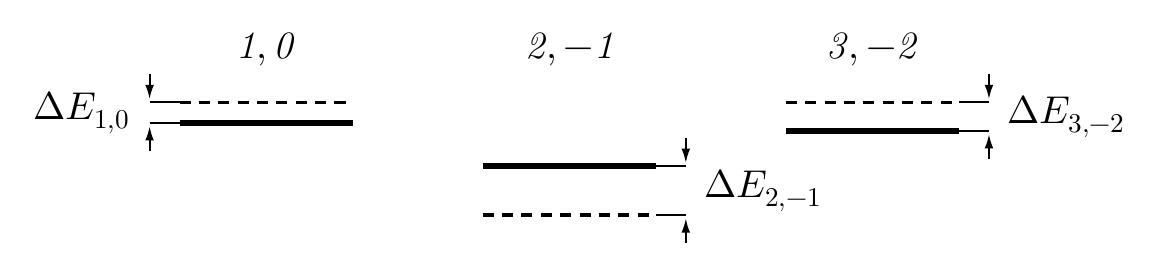
\begin{tikzpicture}[x=1cm,y=1cm]
\def\BareOne{1.40}
\def\IntermediateGap{.55}
% R36 p.95 (9.24), for Delta_2>0:
%   dE_1,0 = + hbar*Omega_12^2/(4 Delta_2) = +a
%   dE_2,-1= - hbar*(Omega_12^2+Omega_23^2)/(4 Delta_2)=-(a+b)
%   dE_3,-2= + hbar*Omega_23^2/(4 Delta_2) = +b
% a=.26 and b=.36 are layout distances only, not spectroscopic values.
\def\StarkA{.26}
\def\StarkB{.36}
\pgfmathsetmacro\ShiftOne{\StarkA}
\pgfmathsetmacro\ShiftThree{\StarkB}
\def\HalfLevel{1.10}
\def\DimensionTail{.36}
\pgfmathsetmacro\BareTwo{\BareOne-\IntermediateGap}
\pgfmathsetmacro\BareThree{\BareOne+\ShiftOne-\ShiftThree}
\pgfmathsetmacro\ShiftTwo{-\ShiftOne-\ShiftThree}
\pgfmathsetmacro\NewOne{\BareOne+\ShiftOne}
\pgfmathsetmacro\NewTwo{\BareTwo+\ShiftTwo}
\pgfmathsetmacro\NewThree{\BareThree+\ShiftThree}
\coordinate (One) at (2.15,\BareOne);
\coordinate (Two) at (6.00,\BareTwo);
\coordinate (Three) at (9.85,\BareThree);
\coordinate (OneShifted) at (2.15,\NewOne);
\coordinate (TwoShifted) at (6.00,\NewTwo);
\coordinate (ThreeShifted) at (9.85,\NewThree);
\foreach \name/\text in {One/{1,0},Two/{2,-1},Three/{3,-2}}{
  \coordinate (\name L) at ($(\name)+(-\HalfLevel,0)$);
  \coordinate (\name R) at ($(\name)+(\HalfLevel,0)$);
  \coordinate (\name SL) at ($(\name Shifted)+(-\HalfLevel,0)$);
  \coordinate (\name SR) at ($(\name Shifted)+(\HalfLevel,0)$);
  \draw[level] (\name L)--(\name R);
  \draw[virtual] (\name SL)--(\name SR);
  \node[levlab,anchor=south] at (\name |- 0,2.04) {$\mathit{\text}$};
}
% CP08: correct source-oriented delta E arrows. Each endpoint has a short
% printed clearance (shorten >= 1.2pt), and no arrow is drawn through a level.
% Exterior, inward-pointing dimension arrows: each meets its own extension line.
\coordinate (D1b) at ($(OneL)+(-.38,0)$);
\coordinate (D1s) at ($(OneSL)+(-.38,0)$);
\draw[baseline] (D1b)--(OneL); \draw[baseline] (D1s)--(OneSL);
\draw[dim] ($(D1b)+(0,-\DimensionTail)$)--(D1b);
\draw[dim] ($(D1s)+(0,\DimensionTail)$)--(D1s);
\node[levlab,anchor=east] at ($(D1b)!.5!(D1s)+(-.16,0)$) {$\Delta E_{1,0}$};
\coordinate (D2b) at ($(TwoR)+(.38,0)$);
\coordinate (D2s) at ($(TwoSR)+(.38,0)$);
\draw[baseline] (TwoR)--(D2b); \draw[baseline] (TwoSR)--(D2s);
\draw[dim] ($(D2b)+(0,\DimensionTail)$)--(D2b);
\draw[dim] ($(D2s)+(0,-\DimensionTail)$)--(D2s);
\node[levlab,anchor=west] at ($(D2b)!.5!(D2s)+(.16,0)$) {$\Delta E_{2,-1}$};
\coordinate (D3b) at ($(ThreeR)+(.38,0)$);
\coordinate (D3s) at ($(ThreeSR)+(.38,0)$);
\draw[baseline] (ThreeR)--(D3b); \draw[baseline] (ThreeSR)--(D3s);
\draw[dim] ($(D3b)+(0,-\DimensionTail)$)--(D3b);
\draw[dim] ($(D3s)+(0,\DimensionTail)$)--(D3s);
\node[levlab,anchor=west] at ($(D3b)!.5!(D3s)+(.16,0)$) {$\Delta E_{3,-2}$};
% Numeric readback for automated checks; no approximate coordinate parsing is needed.
\typeout{FIG93-CHECK BareOne=\BareOne, BareTwo=\BareTwo, BareThree=\BareThree}
\typeout{FIG93-CHECK NewOne=\NewOne, NewTwo=\NewTwo, NewThree=\NewThree}
\end{tikzpicture}

\end{document}
